\documentclass[tikz,border=12pt]{standalone}
\usepackage[T1]{fontenc}
\usepackage{tgheros}
\usepackage{sfmath}
\usepackage{amsmath}
% % \usepackage{fontawesome5} (Removed for publication-grade academic typography) (Removed for publication-grade academic typography)
\usepackage{tikz}
\usetikzlibrary{arrows.meta,positioning,shapes.geometric,fit,backgrounds,calc}
\usepackage{xcolor}

\renewcommand{\familydefault}{\sfdefault}

% Harvard Crimson & ETH Zurich Academic Semantic Palette
\definecolor{harvardcrimson}{HTML}{A51C30}
\definecolor{ethdarkblue}{HTML}{1F407A}
\definecolor{ethblue}{HTML}{215CAF}
\definecolor{ethpetrol}{HTML}{007A87}
\definecolor{ethbronze}{HTML}{B87333}
\definecolor{ethslate}{HTML}{475569}
\definecolor{cardbg}{HTML}{F8FAFC}
\definecolor{cardborder}{HTML}{CBD5E1}
\definecolor{safeTeal}{HTML}{10B981}

\begin{document}
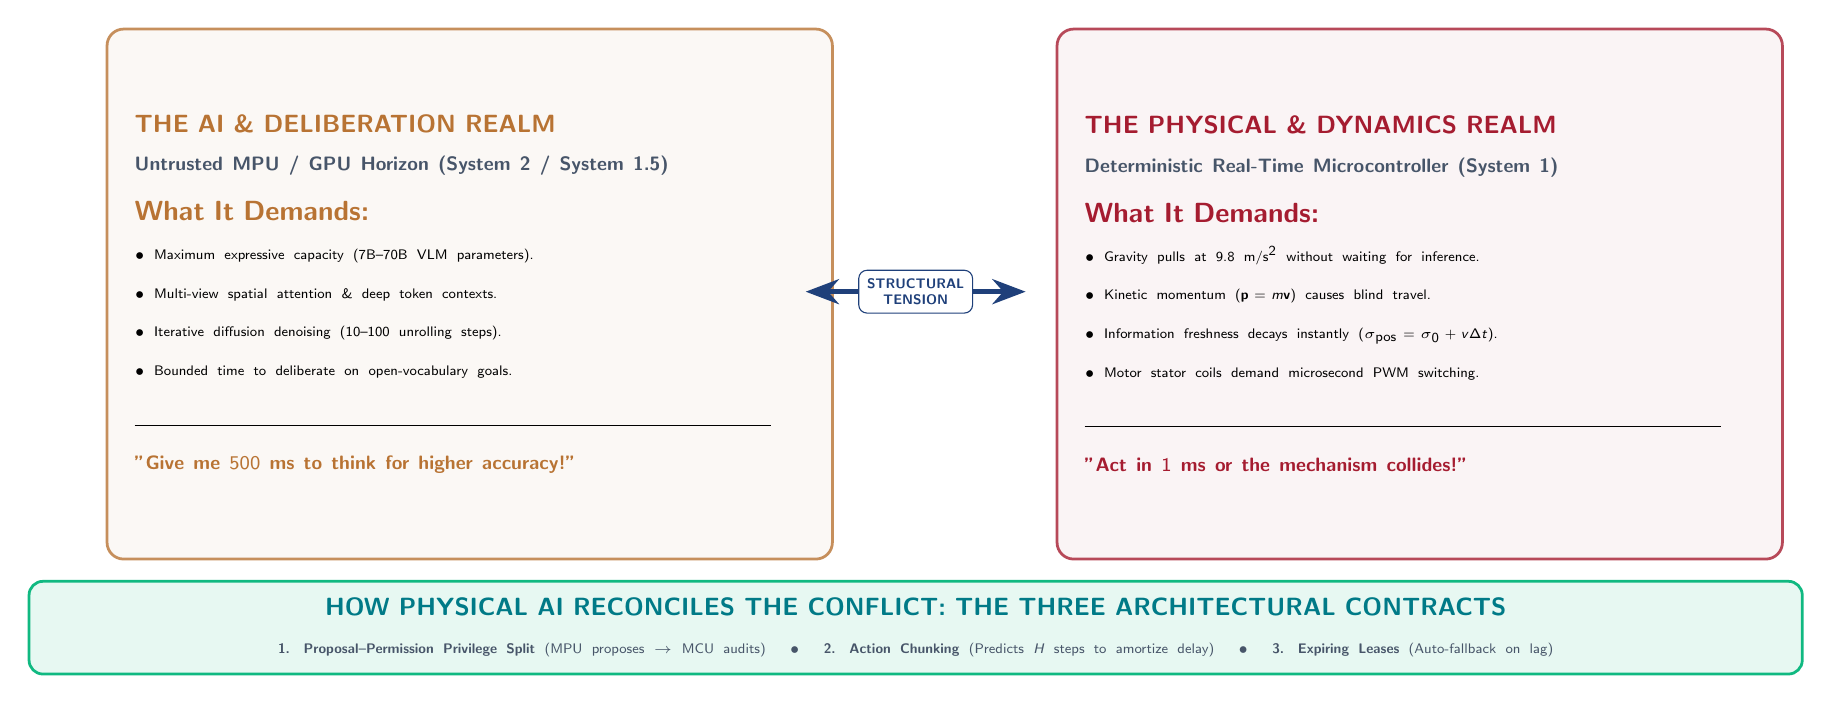
\begin{tikzpicture}[
  font=\sffamily,
  >=Stealth,
  realmcard/.style={
    draw=cardborder,
    fill=cardbg,
    rounded corners=6pt,
    line width=1pt,
    text width=3.35in,
    minimum height=2.65in,
    inner sep=10pt,
    align=left,
    anchor=north west
  }
]

  % Top Title Banner
  % (Top title banner removed for academic publication standards)
% Left Card: The AI / Reasoning Realm (Explicit anchor=north west)
  \node[realmcard, draw=ethbronze!80, fill=ethbronze!5] (ai_realm) at (0.30in, 0.00in) {
    {\small\bfseries\color{ethbronze} THE AI \& DELIBERATION REALM}\\[2pt]
    {\scriptsize\bfseries\color{ethslate}Untrusted MPU / GPU Horizon (System 2 / System 1.5)}\\[6pt]
    \textbf{\color{ethbronze}What It Demands:}\\[2pt]
    {\tiny $\bullet$ Maximum expressive capacity ($7\text{B}\text{--}70\text{B}$ VLM parameters).}\\[2pt]
    {\tiny $\bullet$ Multi-view spatial attention \& deep token contexts.}\\[2pt]
    {\tiny $\bullet$ Iterative diffusion denoising (10--100 unrolling steps).}\\[2pt]
    {\tiny $\bullet$ Bounded time to deliberate on open-vocabulary goals.}\\[6pt]
    \rule{0.95\linewidth}{0.3pt}\\[4pt]
    {\scriptsize\textbf{\color{ethbronze}"Give me $500\text{ ms}$ to think for higher accuracy!"}}
  };

  % Right Card: The Physical / Dynamics Realm (Explicit anchor=north west)
  \node[realmcard, draw=harvardcrimson!80, fill=harvardcrimson!5] (phys_realm) at (5.05in, 0.00in) {
    {\small\bfseries\color{harvardcrimson} THE PHYSICAL \& DYNAMICS REALM}\\[2pt]
    {\scriptsize\bfseries\color{ethslate}Deterministic Real-Time Microcontroller (System 1)}\\[6pt]
    \textbf{\color{harvardcrimson}What It Demands:}\\[2pt]
    {\tiny $\bullet$ Gravity pulls at $9.8\text{ m/s}^2$ without waiting for inference.}\\[2pt]
    {\tiny $\bullet$ Kinetic momentum ($\mathbf{p} = m\mathbf{v}$) causes blind travel.}\\[2pt]
    {\tiny $\bullet$ Information freshness decays instantly ($\sigma_{\text{pos}} = \sigma_0 + v\Delta t$).}\\[2pt]
    {\tiny $\bullet$ Motor stator coils demand microsecond PWM switching.}\\[6pt]
    \rule{0.95\linewidth}{0.3pt}\\[4pt]
    {\scriptsize\textbf{\color{harvardcrimson}"Act in $1\text{ ms}$ or the mechanism collides!"}}
  };

  % Center Tension Tug-of-War Vector (Aligned with badge)
  \draw[<->, line width=2.0pt, draw=ethdarkblue] (3.80in, -1.32in) -- (4.90in, -1.32in);
  \node[font=\sffamily\bfseries\tiny, fill=white, draw=ethdarkblue, rounded corners=3pt, inner sep=3pt, text=ethdarkblue, align=center] at (4.35in, -1.32in) {
    STRUCTURAL\\TENSION
  };

  % Bottom Synthesis Resolution Banner
  \node[draw=safeTeal, fill=safeTeal!10, rounded corners=5pt, line width=1pt, text width=8.70in, inner sep=6pt, align=center] (synthesis) at (4.35in, -3.00in) {
    {\small\bfseries\color{ethpetrol} HOW PHYSICAL AI RECONCILES THE CONFLICT: THE THREE ARCHITECTURAL CONTRACTS}\\[2pt]
    {\tiny\color{ethslate}\textbf{1. Proposal--Permission Privilege Split} (MPU proposes $\to$ MCU audits) $\quad\bullet\quad$ \textbf{2. Action Chunking} (Predicts $H$ steps to amortize delay) $\quad\bullet\quad$ \textbf{3. Expiring Leases} (Auto-fallback on lag)}
  };

\end{tikzpicture}
\end{document}
